\begin{figure*}
	\begin{center}
		\vspace{-0.5in}
		%\hspace*{-2.3cm}
		\setlength{\tabcolsep}{3pt}
		
		\hspace{-0.5in}\normalsize{\textsf{BLURRED TRUE MEAN}}  \hspace{5.5cm} \normalsize{\textsf{NORMALIZED RMSE}} 
		\vspace{0.1in}
		
		
%	\begin{tabular}{ c " c}
%		VIDEO 1& VIDEO 2 \\ \thickhline
%		& \vspace{-.1in} \\
%		VIDEO 3 & VIDEO 4
%	\end{tabular}
%	\qquad
%		\begin{tabular}{ c " c}
%		{{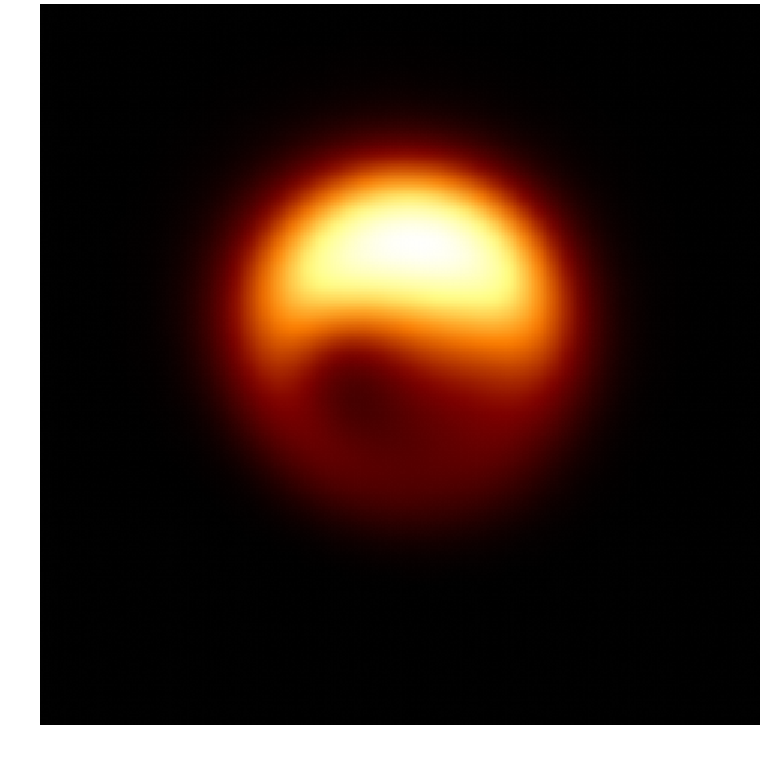
\includegraphics[height=.1\linewidth]{figures/starwarps_results/rotation30/gt/frames/gt_15_blurredbeam75_noaxis.pdf}} } & {{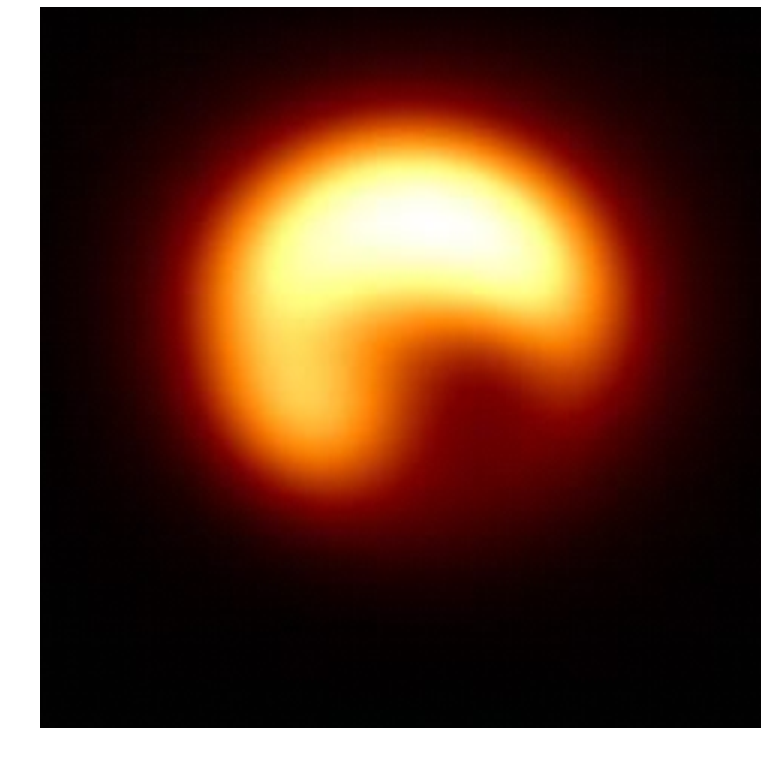
\includegraphics[height=.1\linewidth]{figures/starwarps_results/hotspot100sR2/gt/frames/gt_115_blurredbeam75_noaxis.pdf}} } \\ \thickhline
%		& \vspace{-.1in} \\
%	{{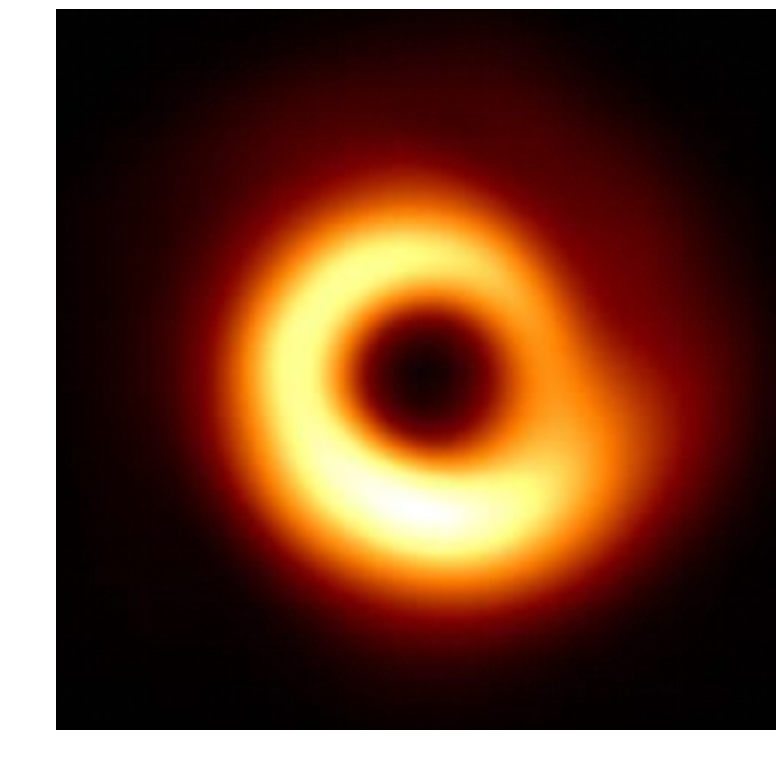
\includegraphics[height=.1\linewidth]{figures/starwarps_results/hotakamovie_02/gt/frames/gt_85_blurredbeam75_noaxis.pdf}} } & {{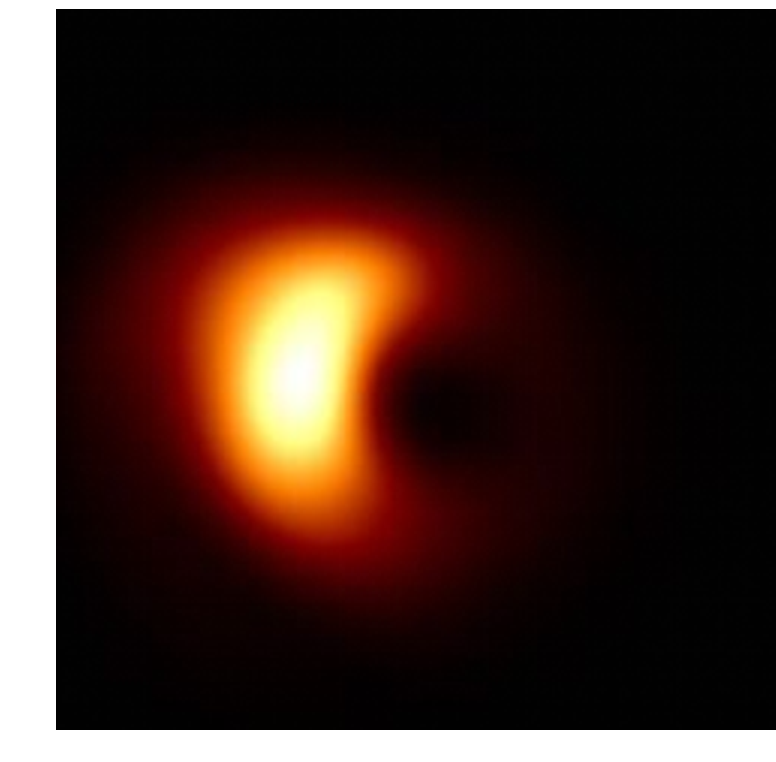
\includegraphics[height=.1\linewidth]{figures/starwarps_results/hotakamovie_45/gt/frames/gt_63_blurredbeam75_noaxis.pdf}} }
%		\end{tabular}
						\begin{tabular}{ c " c}
							\hspace{-.06in} \textsf{Video 1} & \hspace{-.06in} \textsf{Video 2} \\
							{{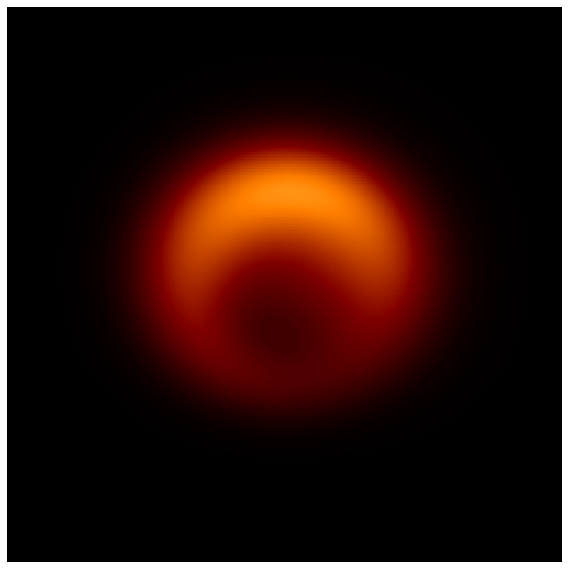
\includegraphics[height=.1\linewidth]{figures/starwarps_results/rotation30/gt/pavgImg_blurredbeam75_noaxis.pdf}} } & {{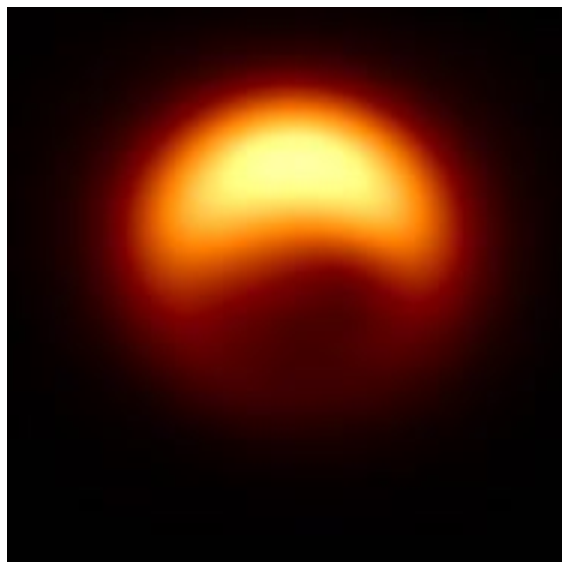
\includegraphics[height=.1\linewidth]{figures/starwarps_results/hotspot100sR2/gt/pavgImg_blurredbeam75_noaxis.pdf}} } \\ \thickhline
							& \vspace{-.1in} \\
							\hspace{-.06in} \textsf{Video 3} & \hspace{-.06in} \textsf{Video 4} \\
							{{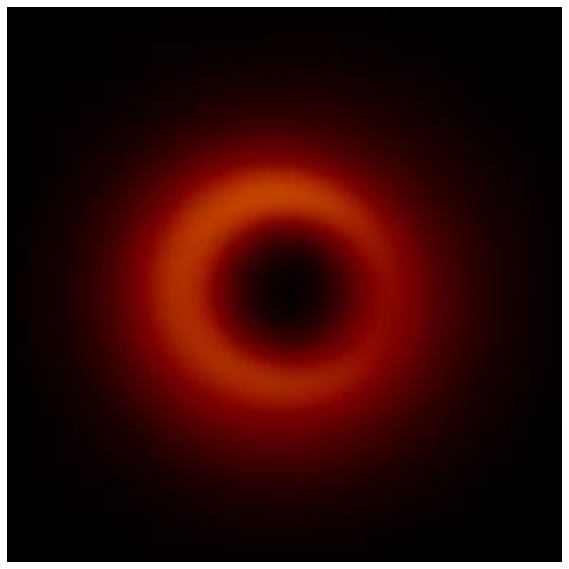
\includegraphics[height=.1\linewidth]{figures/starwarps_results/hotakamovie_02/gt/pavgImg_blurredbeam75_noaxis.pdf}} } & {{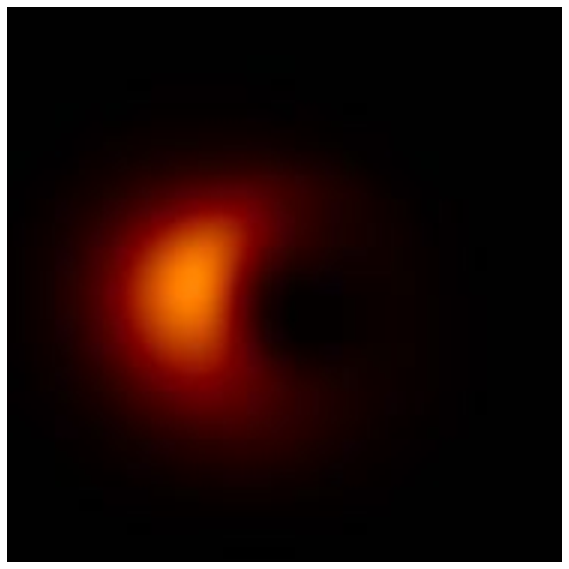
\includegraphics[height=.1\linewidth]{figures/starwarps_results/hotakamovie_45/gt/pavgImg_blurredbeam75_noaxis.pdf}} }
						\end{tabular}	
	%	\qquad	
		\qquad
		\begin{tabular}{ r | c | c | c | c " c | c | c | c}
			& \rotatebox[origin=t]{90}{\small{\textsf{EHT 2017}} } \rotatebox[origin=t]{90}{\small{\textsf{NO ATM.}} }  & \rotatebox[origin=t]{90}{\small{\textsf{EHT 2017}} } \rotatebox[origin=t]{90}{\small{\textsf{ATM.}} } & \rotatebox[origin=t]{90}{\small{\textsf{EHT 2017+}} } \rotatebox[origin=t]{90}{\small{\textsf{ATM.}} } &\rotatebox[origin=t]{90}{\small{\textsf{FUTURE}} } \rotatebox[origin=t]{90}{\small{\textsf{ATM.}} } & \rotatebox[origin=t]{90}{\small{\textsf{EHT 2017}} } \rotatebox[origin=t]{90}{\small{\textsf{NO ATM.}} }  & \rotatebox[origin=t]{90}{\small{\textsf{EHT 2017}} } \rotatebox[origin=t]{90}{\small{\textsf{ATM.}} } & \rotatebox[origin=t]{90}{\small{\textsf{EHT 2017+}} } \rotatebox[origin=t]{90}{\small{\textsf{ATM.}} } &\rotatebox[origin=t]{90}{\small{\textsf{FUTURE}} } \rotatebox[origin=t]{90}{\small{\textsf{ATM.}} }  \\ \hline
			{\small{\textsf{StarWarps Mean} } } & {\bf {0.67} }& {\bf {0.65}} & {\bf {0.55} }&  {\bf {0.55}}& {\bf {0.74}} & {\bf {0.73} }& {\bf {0.73}} &  0.71 \\ 
				\cite{freek} & 1.05  & 0.82 & 0.73  & 0.68 &  0.98 & 1.21 & 0.99 & 0.35 \\ 
				\cite{andrew} & 0.79 & 0.80 & 0.73 & 0.63 & 0.83& 1.05 & 0.81 & {\bf 0.23}  \\  \thickhline
				\small{\textsf{StarWarps Mean} } & {\bf 0.32} & {\bf 0.55} & 0.67 & {\bf 0.36} & {\bf 0.34} & {\bf 0.44} & {\bf 0.23} & {\bf 0.31} \\
				\cite{freek} & 0.93 & 0.90 & {\bf 0.53} & 0.51 & 0.84 & 0.75 & 1.02 & 0.61 \\
				\cite{andrew} &0.84 & 0.85 & 0.71 &  0.39  & 0.60 & 0.50 & 0.60 & 0.47
			\end{tabular}

		\vspace{0.4in}
		
		\hspace*{-1.3cm}
		\begin{tabular}{  c c | c  c  c  c "  c  c  c  c  }
			%\hline
			& \small{\textsf{Array:}} &\small{\textsf{EHT 2017}}   &\small{\textsf{EHT 2017 }} &\small{\textsf{EHT2017+}}    &\small{\textsf{FUTURE}}    &\small{\textsf{EHT 2017}}   &\small{\textsf{EHT 2017 }} &\small{\textsf{EHT2017+}}    &\small{\textsf{FUTURE}}     \\ 
			&\vspace{-.1in} & & & & & & & &\\
			& \small{\textsf{Error:}} &\small{\textsf{NO ATM.}}   &\small{\textsf{ATM.}} &\small{\textsf{ATM.}}    &\small{\textsf{ATM.}}  &\small{\textsf{NO ATM.}}   &\small{\textsf{ATM.}} &\small{\textsf{ATM.}}    &\small{\textsf{ATM.}}   \\ \hline
%			&\vspace{-.1in} & & & & & & & &\\
%			\multirow{2}{*}[0.2in]{ \rotatebox[origin=t]{90}{\small{\textsf{StarWarps}} }}   \hspace{-0.3in} & \multirow{1}{*}[0.5in]{ \rotatebox[origin=t]{90}{\small{\textsf{FRAME}} }}
%			&
%			{{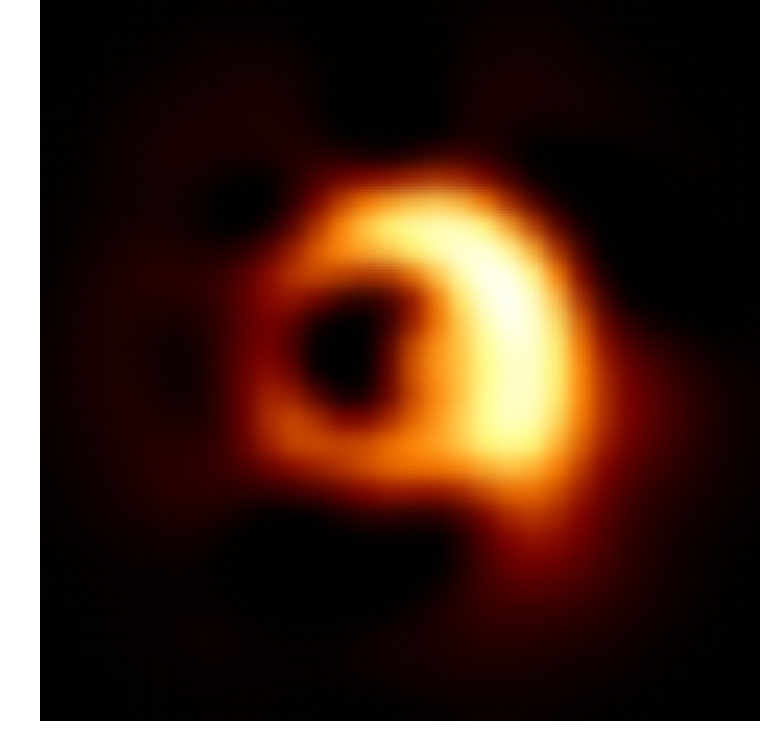
\includegraphics[height=.1\linewidth]{figures/starwarps_results/rotation30/eht2017_100_visibility/nomotion/frames/mean_noaxis_15.pdf}} } &
%			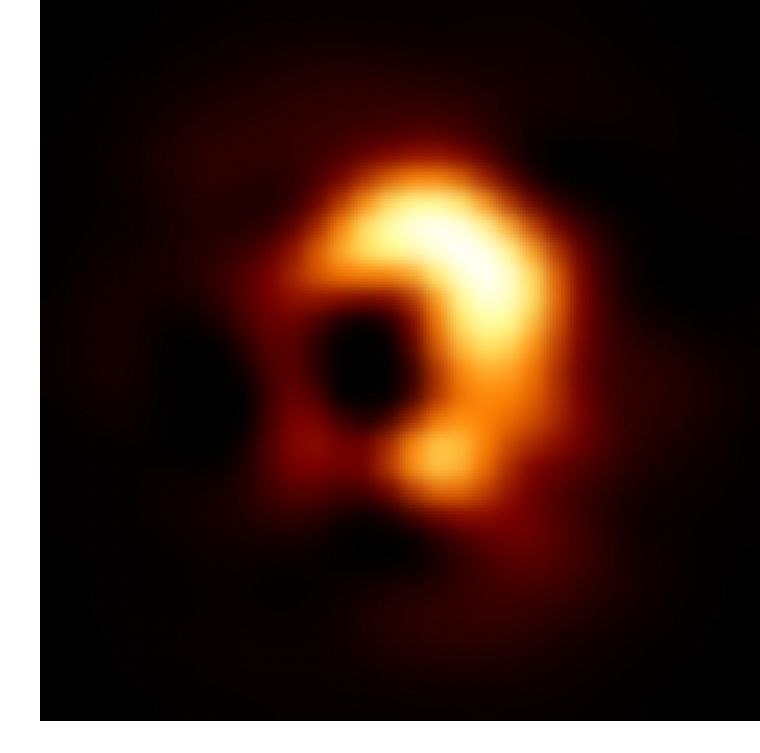
\includegraphics[height=.1\linewidth]{figures/starwarps_results/rotation30/eht2017_100_amp-bispectrum/nomotion/frames/mean_noaxis_15.pdf} &
%			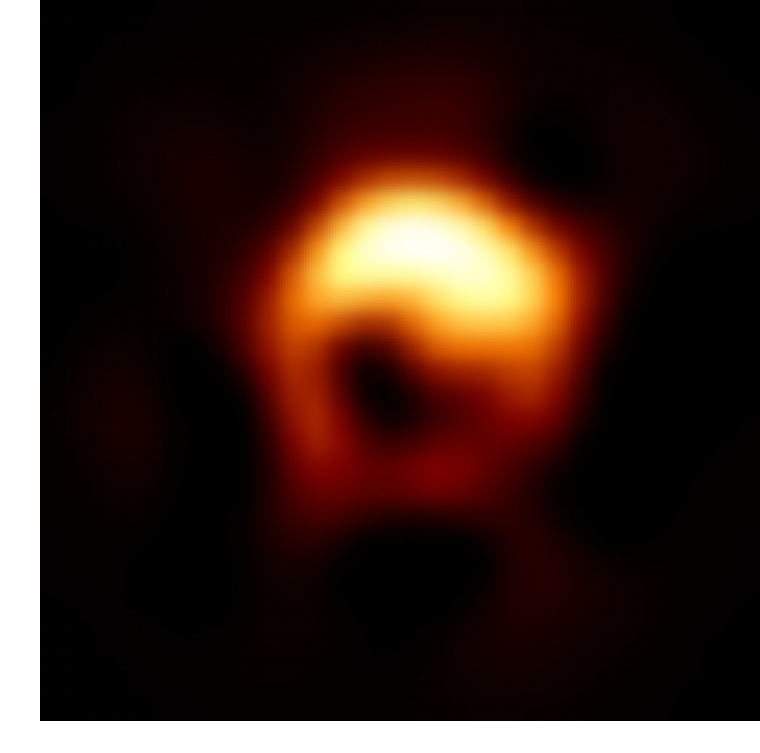
\includegraphics[height=.1\linewidth]{figures/starwarps_results/rotation30/ehtfuture2_100_amp-bispectrum/nomotion/frames/mean_noaxis_15.pdf} &
%			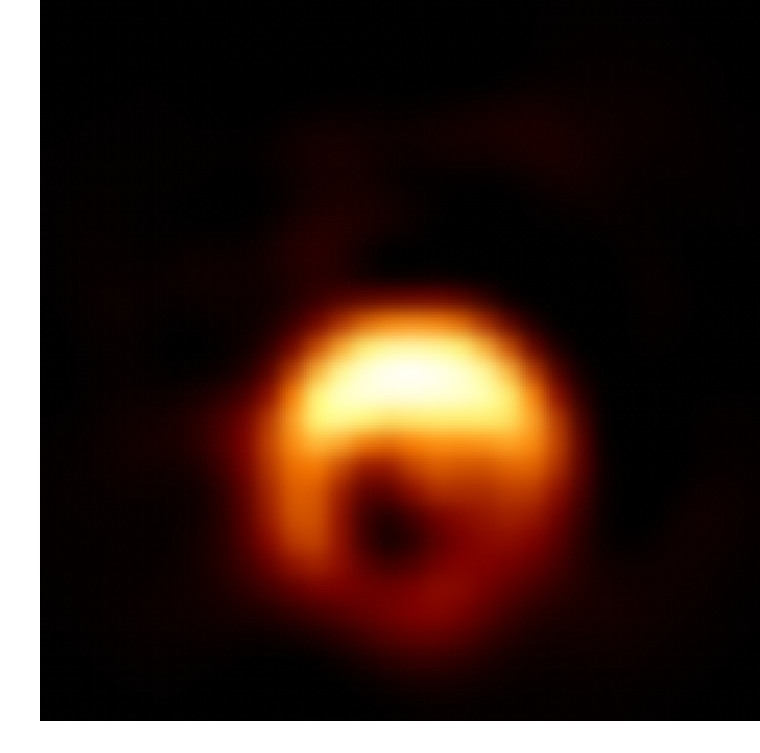
\includegraphics[height=.1\linewidth]{figures/starwarps_results/rotation30/ehtfuture1_100_amp-bispectrum/nomotion/frames/mean_noaxis_15.pdf}  
%			&
%			{{\includegraphics[height=.1\linewidth]{figures/starwarps_results/hotspot100sR2/eht2017_100_visibility/nomotion/frames/mean_noaxis_115.pdf}} } &
%			\includegraphics[height=.1\linewidth]{figures/starwarps_results/hotspot100sR2/eht2017_100_amp-bispectrum/nomotion/frames/mean_noaxis_115.pdf} &
%			\includegraphics[height=.1\linewidth]{figures/starwarps_results/hotspot100sR2/ehtfuture2_100_amp-bispectrum/nomotion/frames/mean_noaxis_115.pdf} &
%			\includegraphics[height=.1\linewidth]{figures/starwarps_results/hotspot100sR2/ehtfuture1_100_amp-bispectrum/nomotion/frames/mean_noaxis_115.pdf} \\
			&\vspace{-.1in} & & & & & & & &\\
			 \multirow{2}{*}[0.6in]{ \rotatebox[origin=t]{90}{\small{\textsf{StarWarps}} }}   \hspace{-0.3in} &	\multirow{1}{*}[0.45in]{ \rotatebox[origin=t]{90}{\small{\textsf{Mean}} }}
			&
			{{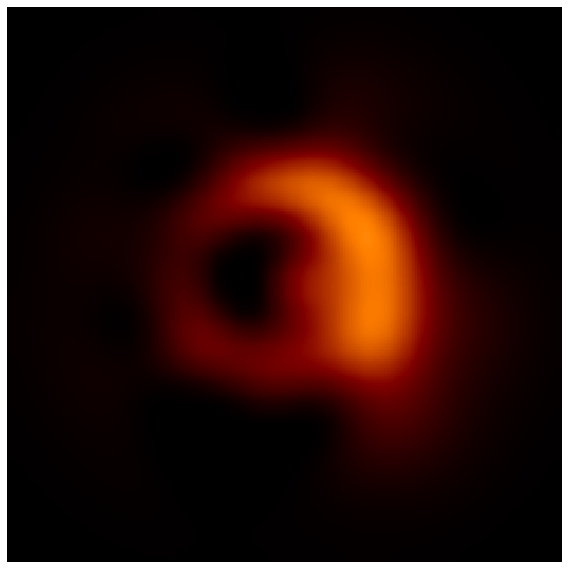
\includegraphics[height=.1\linewidth]{figures/starwarps_results/rotation30/eht2017_100_visibility/nomotion/pavgimg_noaxis.pdf}} } &
			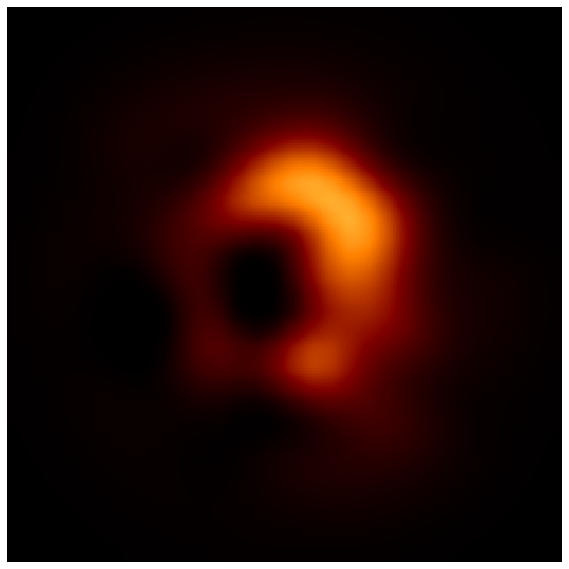
\includegraphics[height=.1\linewidth]{figures/starwarps_results/rotation30/eht2017_100_amp-bispectrum/nomotion/pavgimg_noaxis.pdf} &
			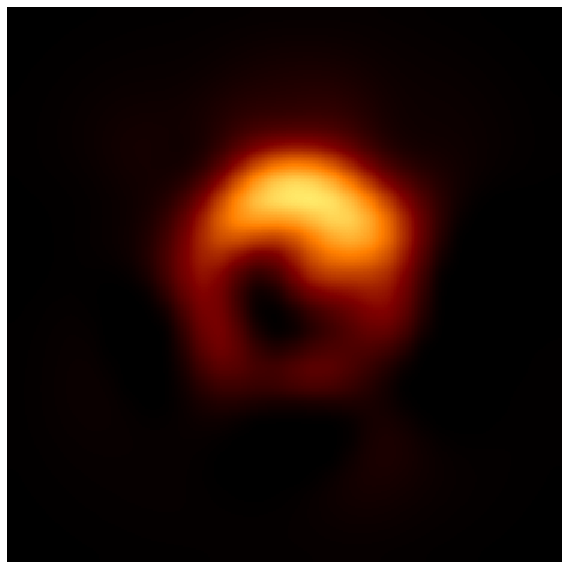
\includegraphics[height=.1\linewidth]{figures/starwarps_results/rotation30/ehtfuture2_100_amp-bispectrum/nomotion/pavgimg_noaxis.pdf} &
			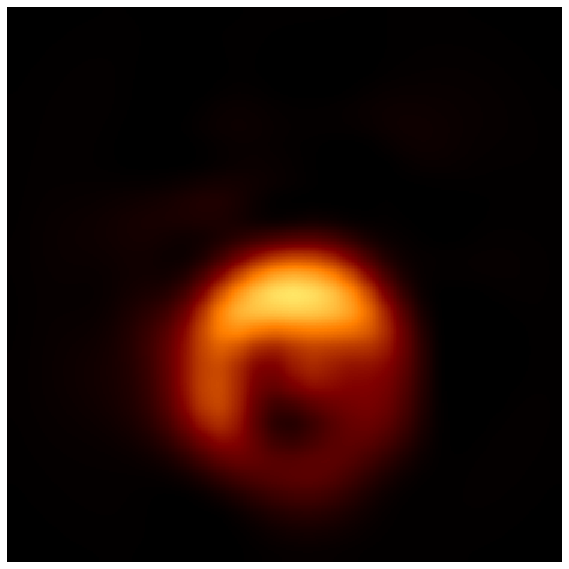
\includegraphics[height=.1\linewidth]{figures/starwarps_results/rotation30/ehtfuture1_100_amp-bispectrum/nomotion/pavgimg_noaxis.pdf} 
			&
			{{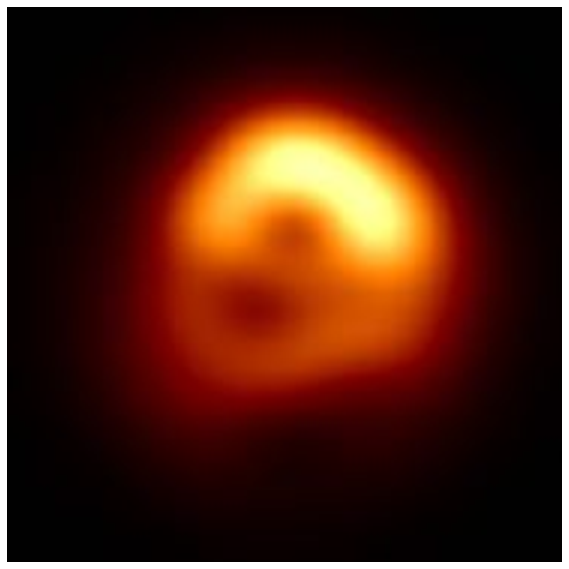
\includegraphics[height=.1\linewidth]{figures/starwarps_results/hotspot100sR2/eht2017_100_visibility/nomotion/pavgimg_noaxis.pdf}} } &
			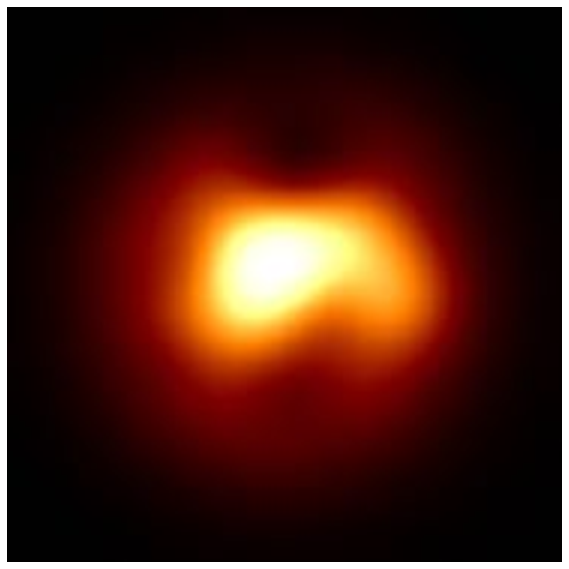
\includegraphics[height=.1\linewidth]{figures/starwarps_results/hotspot100sR2/eht2017_100_amp-bispectrum/nomotion/pavgimg_noaxis.pdf} &
			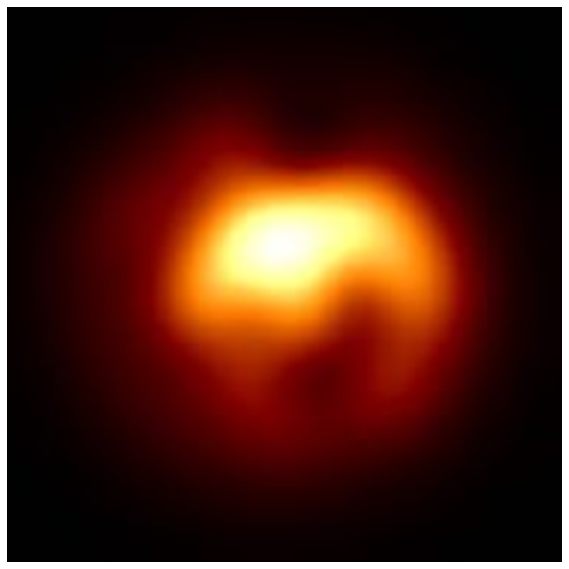
\includegraphics[height=.1\linewidth]{figures/starwarps_results/hotspot100sR2/ehtfuture2_100_amp-bispectrum/nomotion/pavgimg_noaxis.pdf} &
			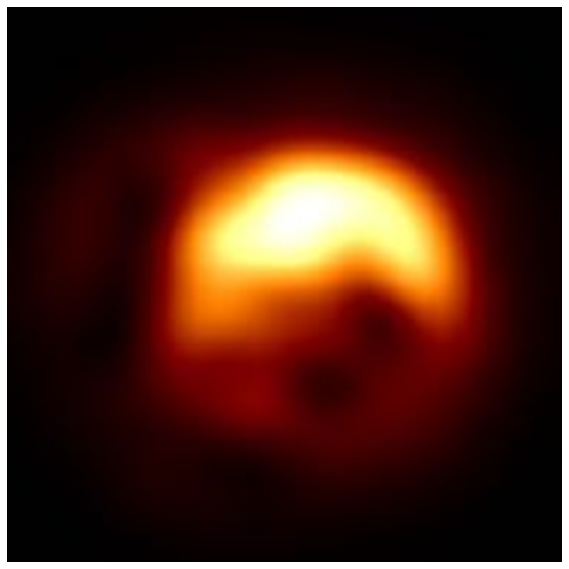
\includegraphics[height=.1\linewidth]{figures/starwarps_results/hotspot100sR2/ehtfuture1_100_amp-bispectrum/nomotion/pavgimg_noaxis.pdf} 
			\\   \hline
			&\vspace{-.1in} & & & & & & & &\\
			\multirow{2}{*}[0.6in]{ \rotatebox[origin=t]{90}{\small{\textsf{MEM \& TV Regularization}} }}  \hspace{-0.3in} & \multirow{1}{*}[0.4in]{ \rotatebox[origin=t]{90}{\small{\textsf{\cite{freek}}} }}
			&
			{{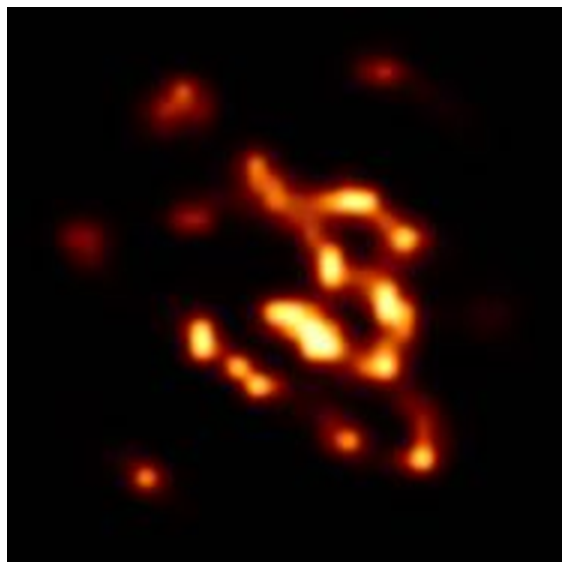
\includegraphics[height=.1\linewidth]{figures/freeksmoothingresults/im_vis_rotation30_tint100_eht2017_directim_maxit100_it0.pdf}} } &
			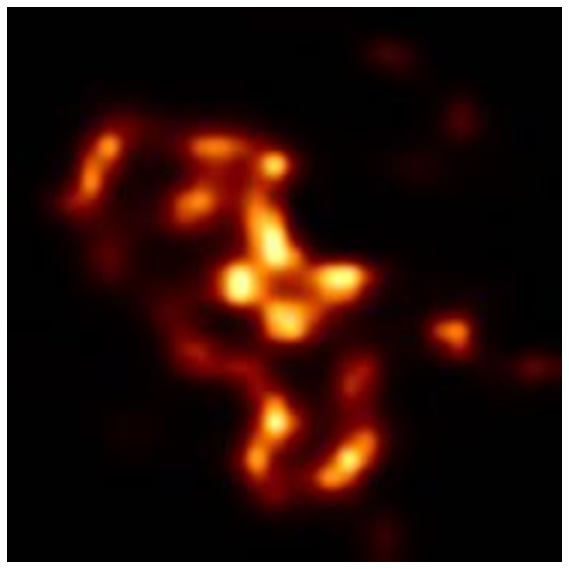
\includegraphics[height=.1\linewidth]{figures/freeksmoothingresults/im_apar_rotation30_tint100_eht2017_directim_maxit100_it0.pdf} &
			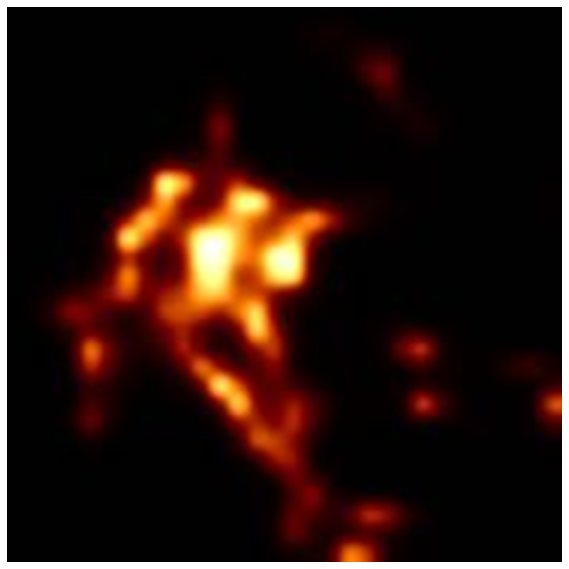
\includegraphics[height=.1\linewidth]{figures/freeksmoothingresults/im_apar_rotation30_tint100_ehtfuture2_directim_maxit100_it0.pdf} &
			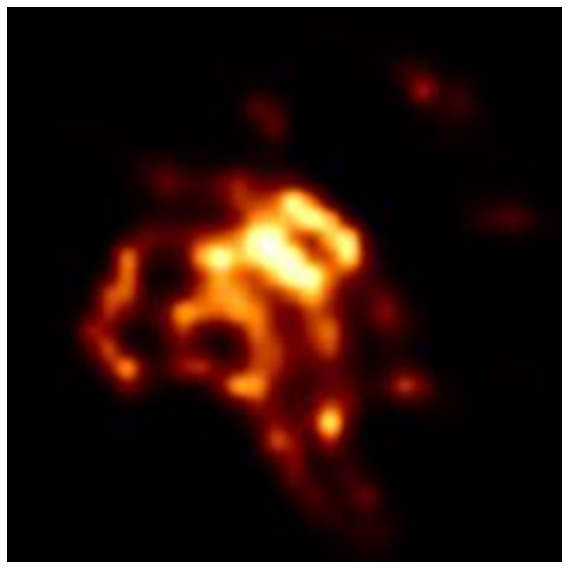
\includegraphics[height=.1\linewidth]{figures/freeksmoothingresults/im_apar_rotation30_tint100_ehtfuture1_directim_maxit100_it0.pdf} 
			&
			{{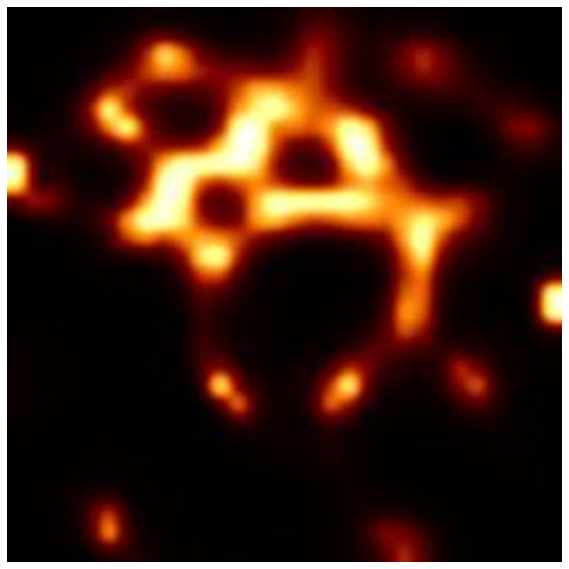
\includegraphics[height=.1\linewidth]{figures/freeksmoothingresults/im_vis_hotspot100sR2_tint100_eht2017_directim_maxit100_it0.pdf}} } &
			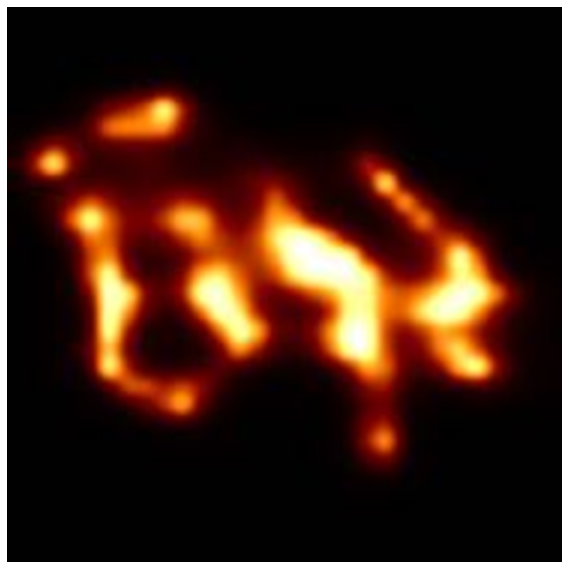
\includegraphics[height=.1\linewidth]{figures/freeksmoothingresults/im_apar_hotspot100sR2_tint100_eht2017_directim_maxit100_it0.pdf} &
			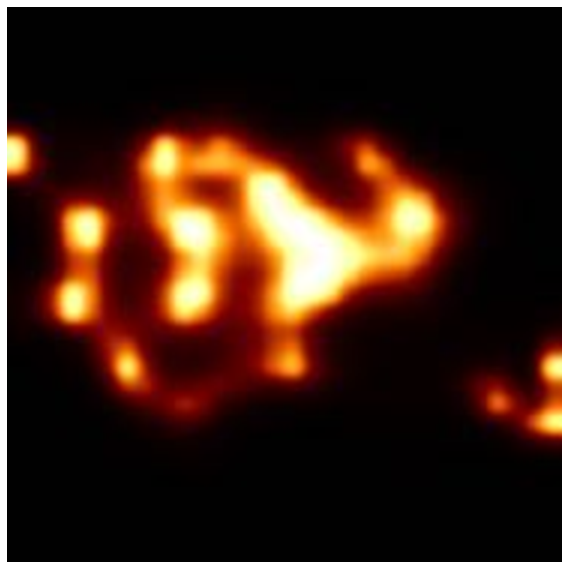
\includegraphics[height=.1\linewidth]{figures/freeksmoothingresults/im_apar_hotspot100sR2_tint100_ehtfuture2_directim_maxit100_it0.pdf} &
			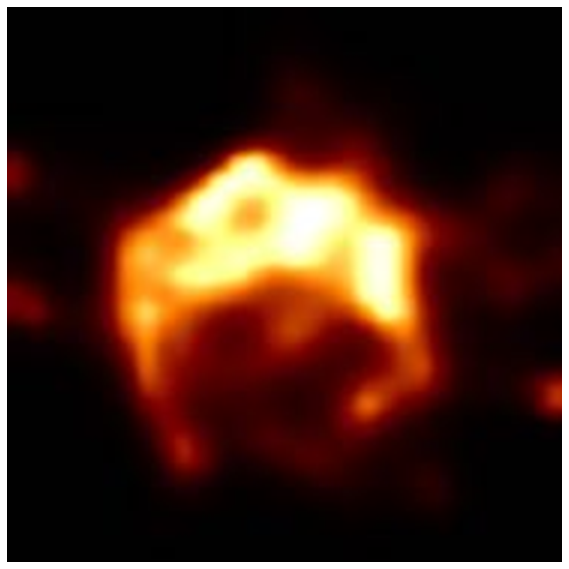
\includegraphics[height=.1\linewidth]{figures/freeksmoothingresults/im_apar_hotspot100sR2_tint100_ehtfuture1_directim_maxit100_it0.pdf} 
			\\
			&\vspace{-.1in} & & & & & & & &\\
			&	\multirow{1}{*}[0.4in]{ \rotatebox[origin=t]{90}{\small{\textsf{\cite{andrew}}} }}
			&
			{{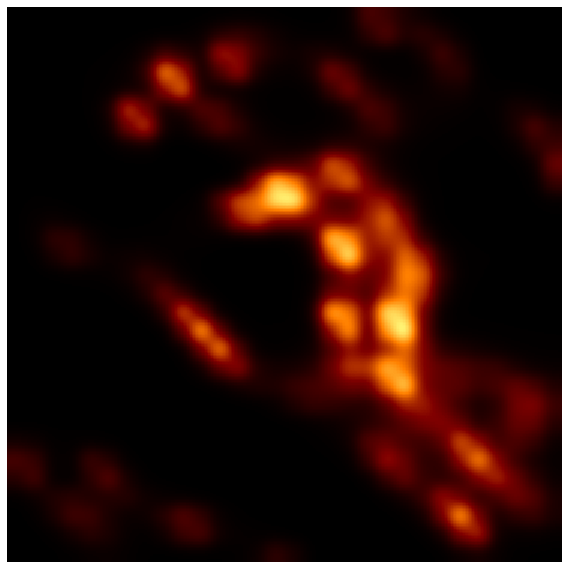
\includegraphics[height=.1\linewidth]{figures/starwarps_results/rotation30/eht2017_100_compare/none_vis_blur025.pdf}} } &
			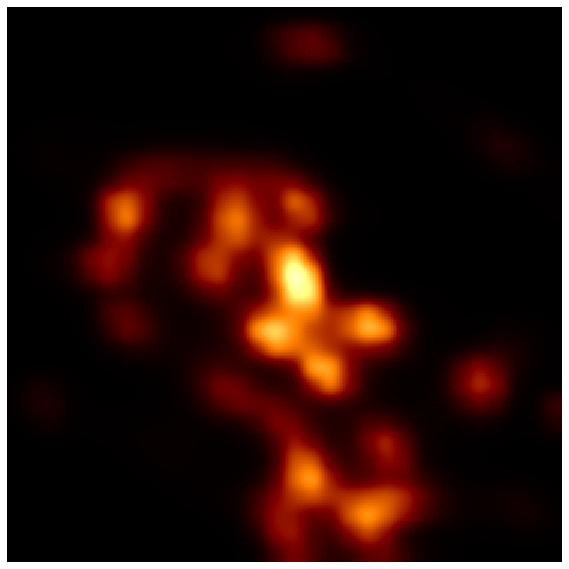
\includegraphics[height=.1\linewidth]{figures/starwarps_results/rotation30/eht2017_100_compare/none_amp-clphase_blur025.pdf} &
			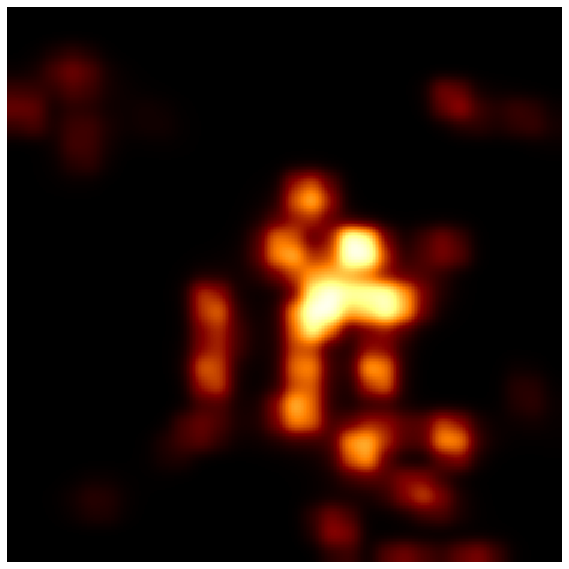
\includegraphics[height=.1\linewidth]{figures/starwarps_results/rotation30/ehtfuture2_100_compare/none_amp-clphase_blur025.pdf} &
			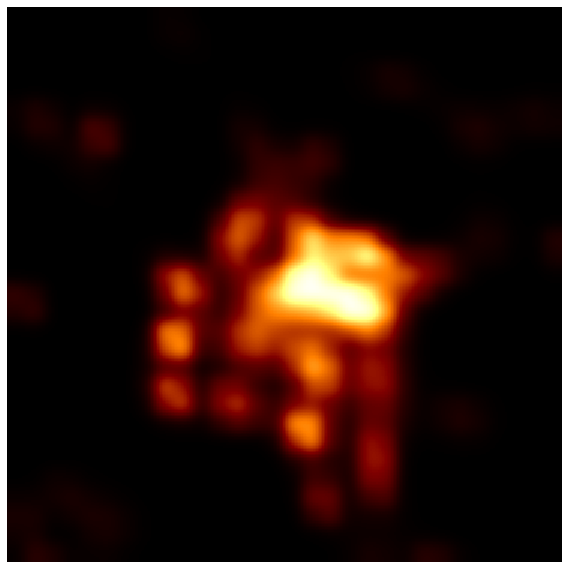
\includegraphics[height=.1\linewidth]{figures/starwarps_results/rotation30/ehtfuture1_100_compare/none_amp-clphase_blur025.pdf} 
			&
			{{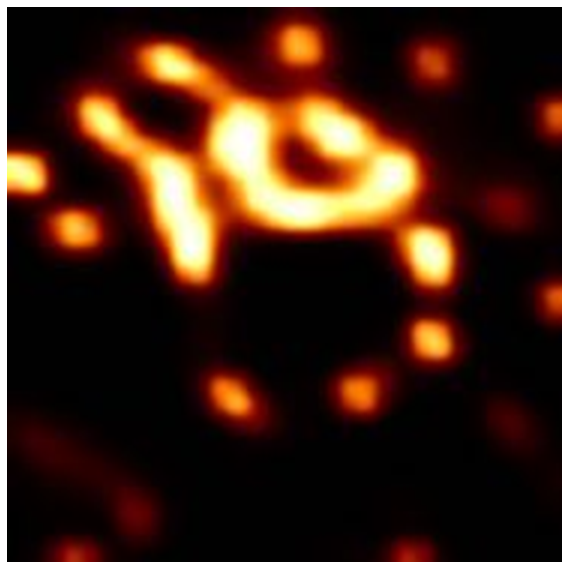
\includegraphics[height=.1\linewidth]{figures/starwarps_results/hotspot100sR2/eht2017_100_compare/none_vis_blur025.pdf}} } &
			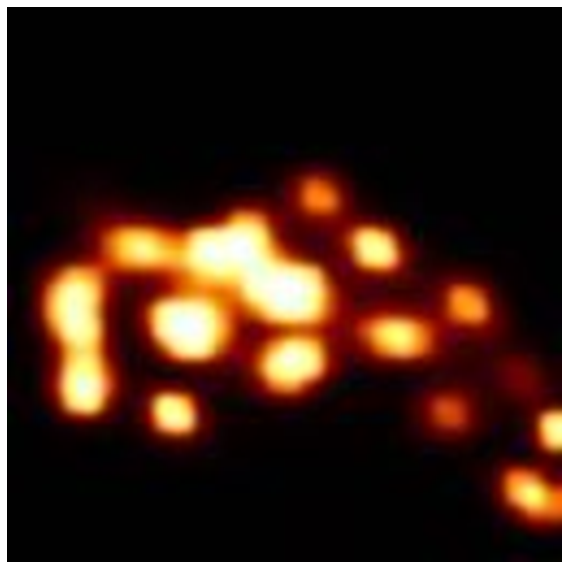
\includegraphics[height=.1\linewidth]{figures/starwarps_results/hotspot100sR2/eht2017_100_compare/none_amp-clphase_blur025.pdf} &
			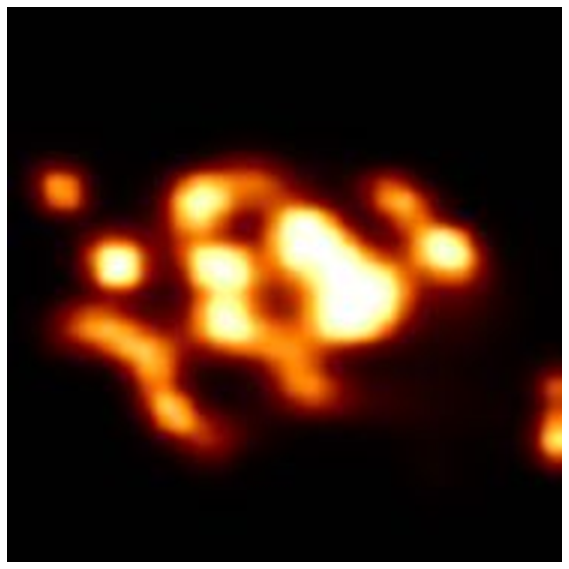
\includegraphics[height=.1\linewidth]{figures/starwarps_results/hotspot100sR2/ehtfuture2_100_compare/none_amp-clphase_blur025.pdf} &
			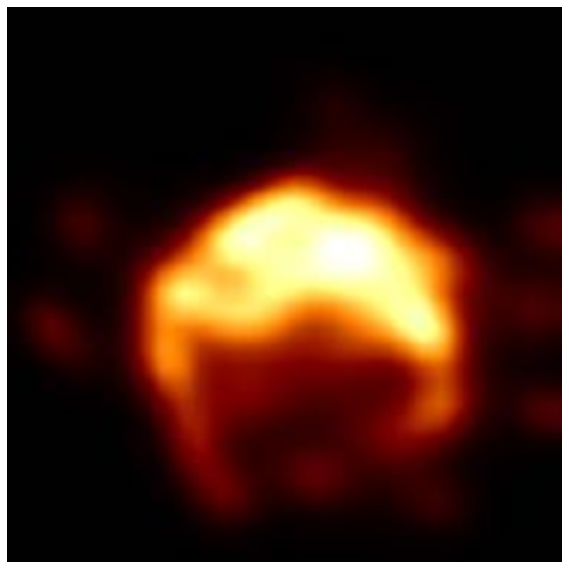
\includegraphics[height=.1\linewidth]{figures/starwarps_results/hotspot100sR2/ehtfuture1_100_compare/none_amp-clphase_blur025.pdf} 
			\\   \thickhline
			
%			&\vspace{-.1in} & & & & & & & &\\
%			\multirow{2}{*}[0.2in]{ \rotatebox[origin=t]{90}{\small{\textsf{StarWarps}} }}  \hspace{-0.3in} & \multirow{1}{*}[0.5in]{ \rotatebox[origin=t]{90}{\small{\textsf{FRAME}} }}
%			&
%			{{\includegraphics[height=.1\linewidth]{figures/starwarps_results/hotakamovie_02/eht2017_100_visibility/nomotion/frames/mean_noaxis_85.pdf}} } &
%			\includegraphics[height=.1\linewidth]{figures/starwarps_results/hotakamovie_02/eht2017_100_amp-bispectrum/nomotion/frames/mean_noaxis_85.pdf} 
%			%\includegraphics[height=.1\linewidth]{figures/starwarps_results/starwarps_hotaka02_2/nomotion/mean_85.png} 
%			&
%			\includegraphics[height=.1\linewidth]{figures/starwarps_results/hotakamovie_02/ehtfuture2_100_amp-bispectrum/nomotion/frames/mean_noaxis_85.pdf} &
%			\includegraphics[height=.1\linewidth]{figures/starwarps_results/hotakamovie_02/ehtfuture1_100_amp-bispectrum/nomotion/frames/mean_noaxis_85.pdf} 
%			&
%			{{\includegraphics[height=.1\linewidth]{figures/starwarps_results/hotakamovie_45/eht2017_100_visibility/nomotion/frames/mean_noaxis_63.pdf}} } &
%			\includegraphics[height=.1\linewidth]{figures/starwarps_results/hotakamovie_45/eht2017_100_amp-bispectrum/nomotion/frames/mean_noaxis_63.pdf} &
%			\includegraphics[height=.1\linewidth]{figures/starwarps_results/hotakamovie_45/ehtfuture2_100_amp-bispectrum/nomotion/frames/mean_noaxis_63.pdf} &
%			\includegraphics[height=.1\linewidth]{figures/starwarps_results/hotakamovie_45/ehtfuture1_100_amp-bispectrum/nomotion/frames/mean_noaxis_63.pdf} \\
			&\vspace{-.1in} & & & & & & & &\\
			 \multirow{2}{*}[0.6in]{ \rotatebox[origin=t]{90}{\small{\textsf{StarWarps}} }}   \hspace{-0.3in} &	\multirow{1}{*}[0.45in]{ \rotatebox[origin=t]{90}{\small{\textsf{Mean}} }}
			&
			{{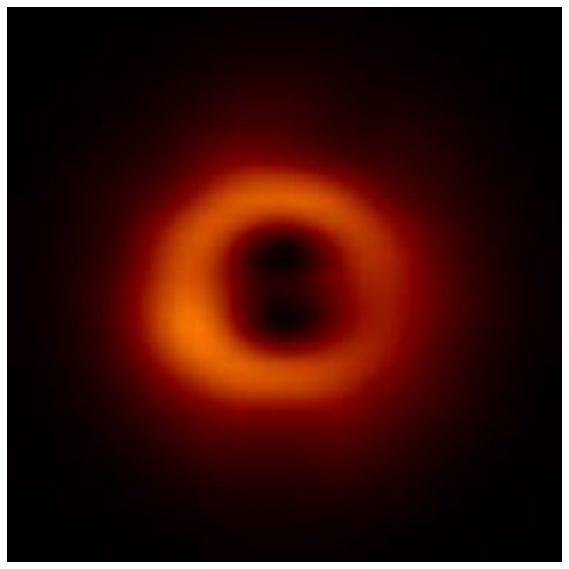
\includegraphics[height=.1\linewidth]{figures/starwarps_results/hotakamovie_02/eht2017_100_visibility/nomotion/pavgimg_noaxis.pdf}} } 
			&
			\includegraphics[height=.1\linewidth]{figures/starwarps_results/hotakamovie_02/eht2017_100_amp-bispectrum/nomotion/pavgimg_noaxis.pdf} 
			%\includegraphics[height=.1\linewidth]{figures/starwarps_results/starwarps_hotaka02_2/avgImg.pdf} 
			&
			\includegraphics[height=.1\linewidth]{figures/starwarps_results/hotakamovie_02/ehtfuture2_100_amp-bispectrum/nomotion/pavgimg_noaxis.pdf} &
			\includegraphics[height=.1\linewidth]{figures/starwarps_results/hotakamovie_02/ehtfuture1_100_amp-bispectrum/nomotion/pavgimg_noaxis.pdf} 
			&
			{{\includegraphics[height=.1\linewidth]{figures/starwarps_results/hotakamovie_45/eht2017_100_visibility/nomotion/pavgimg_noaxis.pdf}} } &
			\includegraphics[height=.1\linewidth]{figures/starwarps_results/hotakamovie_45/eht2017_100_amp-bispectrum/nomotion/pavgimg_noaxis.pdf} &
			\includegraphics[height=.1\linewidth]{figures/starwarps_results/hotakamovie_45/ehtfuture2_100_amp-bispectrum/nomotion/pavgimg_noaxis.pdf} &
			\includegraphics[height=.1\linewidth]{figures/starwarps_results/hotakamovie_45/ehtfuture1_100_amp-bispectrum/nomotion/pavgimg_noaxis.pdf} 
			\\   \hline
			&\vspace{-.1in} & & & & & & & &\\
			\multirow{2}{*}[0.6in]{ \rotatebox[origin=t]{90}{\small{\textsf{MEM \& TV Regularization}} }}  \hspace{-0.3in} & 	\multirow{1}{*}[0.4in]{ \rotatebox[origin=t]{90}{\small{\textsf{\cite{freek}}} }}
			&
			{{\includegraphics[height=.1\linewidth]{figures/freeksmoothingresults/im_vis_hotakamovie_02_16300_20999_tint100_eht2017_directim_maxit100_it0.pdf}} } &
			\includegraphics[height=.1\linewidth]{figures/freeksmoothingresults/im_apar_hotakamovie_02_16300_20999_tint100_eht2017_directim_maxit100_it0.pdf} &
			\includegraphics[height=.1\linewidth]{figures/freeksmoothingresults/im_apar_hotakamovie_02_16300_20999_tint100_ehtfuture2_directim_maxit100_it0.pdf} &
			\includegraphics[height=.1\linewidth]{figures/freeksmoothingresults/im_apar_hotakamovie_02_16300_20999_tint100_ehtfuture1_directim_maxit100_it0.pdf} 
			&
			{{\includegraphics[height=.1\linewidth]{figures/freeksmoothingresults/im_vis_hotakamovie_45_16300_20999_tint100_eht2017_directim_maxit100_it0.pdf}} } &
			\includegraphics[height=.1\linewidth]{figures/freeksmoothingresults/im_apar_hotakamovie_45_16300_20999_tint100_eht2017_directim_maxit100_it0.pdf} &
			\includegraphics[height=.1\linewidth]{figures/freeksmoothingresults/im_apar_hotakamovie_45_16300_20999_tint100_ehtfuture2_directim_maxit100_it0.pdf} &
			\includegraphics[height=.1\linewidth]{figures/freeksmoothingresults/im_apar_hotakamovie_45_16300_20999_tint100_ehtfuture1_directim_maxit100_it0.pdf} 
			\\
			&\vspace{-.1in} & & & & & & & &\\
			&	\multirow{1}{*}[0.4in]{ \rotatebox[origin=t]{90}{\small{\textsf{\cite{andrew}}} }}
			&
			{{\includegraphics[height=.1\linewidth]{figures/starwarps_results/hotakamovie_02/eht2017_100_compare/none_vis_blur025.pdf}} } &
			\includegraphics[height=.1\linewidth]{figures/starwarps_results/hotakamovie_02/eht2017_100_compare/none_amp-clphase_blur025.pdf} 
			&
			\includegraphics[height=.1\linewidth]{figures/starwarps_results/hotakamovie_02/ehtfuture2_100_compare/none_amp-clphase_blur025.pdf} &
			\includegraphics[height=.1\linewidth]{figures/starwarps_results/hotakamovie_02/ehtfuture1_100_compare/none_amp-clphase_blur025.pdf} 
			&
			{{\includegraphics[height=.1\linewidth]{figures/starwarps_results/hotakamovie_45/eht2017_100_compare/none_vis_blur025.pdf}} } &
			\includegraphics[height=.1\linewidth]{figures/starwarps_results/hotakamovie_45/eht2017_100_compare/none_amp-clphase_blur025.pdf} &
			\includegraphics[height=.1\linewidth]{figures/starwarps_results/hotakamovie_45/ehtfuture2_100_compare/none_amp-clphase_blur025.pdf} &
			\includegraphics[height=.1\linewidth]{figures/starwarps_results/hotakamovie_45/ehtfuture1_100_compare/none_amp-clphase_blur025.pdf} 
			\\ 
		\end{tabular}
		\caption{\scriptsize{\bf Static evolution model:} Results obtained using data simulated from each of the 4 video sequences (see Figure~\ref{fig:groundtruth}) under different telescope arrays (see Figures~\ref{fig:staticimaging} and~\ref{fig:uvcov2}) and noise conditions. The main portion of the figure is broken up into 4 quadrants corresponding to Videos 1-4 when moving from left to right, top to bottom. The true mean image from the ground truth videos, blurred to 3/4 the nominal resolution of the array, is shown on the top. We compare results of our proposed method, StarWarps, to that of the single imaging methods presented in~\cite{freek} and~\cite{andrew}. In particular, we compare the mean image obtained using StarWarps video reconstruction. The error type NO ATM. indicates reconstructing using visibilities on data with no atmospheric error, while the error type ATM. indicates using the visibility amplitudes and bispectrum on data where atmospheric phase errors have been introduced. The quality of each result, compared to the ground truth mean image, is indicated in the table of normalized root mean squared errors (Normalized RMSE). To account for the loss of absolute position in the presence of atmospheric phase error, images were rigidly aligned to the true mean before computing the error. The FOV and colorbar used for each reconstruction can be seen in Figure~\ref{fig:groundtruth}. }
		\label{fig:staticevolutionresults}
	\end{center}
\end{figure*}



























































